\documentclass{egee}
\usepackage{comment,alltt}

\def\LB{L\&B}

\title{gLite Job Provenance Install Guide}
\author{CESNET EGEE JRA1 team}
\DocIdentifier{EGEE-JRA1-??}
\Date{\today}
\Activity{JRA1: Middleware Engineering and Integration}
\DocStatus{DRAFT}
\Dissemination{PUBLIC}
\DocumentLink{}
\Abstract{This install guide of the Job Provenance (JP) service is
  intended as a detailed technical guide to the JP deployment process
  (including all configuration tasks on related services). 
  For description of deployment modules please refer to the "gLite
  install guide" document. 
 
  Currently this document contains only description of LB-JP
  interaction internals. 
}


\def\todo#1{\textbf{TODO:} #1}

\begin{document}


%\begin{center}
{\bf Delivery Slip}
\end{center}
\begin{tabularx}{\textwidth}{|l|l|l|X|X|}
\hline
           & {\bf Name} & {\bf Partner} & {\bf Date} & {\bf Signature} \\
\hline
{\bf From} &                  &  & & \\
\hline
{\bf Reviewed by} & &  & & \\

\hline
{\bf Approved by} & & & & \\
\hline
\end{tabularx}

\begin{center}
{\bf Document Change Log}
\end{center}

\begin{tabularx}{\textwidth}{|l|l|X|X|}
\hline
{\bf Issue } & {\bf Date  } & {\bf Comment } & {\bf Author  } \\   \hline

\hline
\end{tabularx}

\begin{center}
{\bf Document Change Record}
\end{center}

\begin{tabularx}{\textwidth}{|l|l|X|}
\hline
{\bf Issue } & {\bf Item  } & {\bf Reason for Change } \\   \hline

\hline
\end{tabularx}

%
% Official text received on October 6, 2004
%
\vfill{\bf Copyright }\copyright{\bf Members of the EGEE Collaboration. 2004. 
See http://eu-egee.org/partners for details on the copyright holders. 

EGEE (``Enabling Grids for E-science in Europe'') is a project funded by
the European Union.  For more information on the project, its partners
and contributors please see http://www.eu-egee.org.

You are permitted to copy and distribute verbatim copies of this
document containing this copyright notice, but modifying this document
is not allowed. You are permitted to copy this document in whole or in
part into other documents if you attach the following reference to the
copied elements: ``Copyright }\copyright{\bf 2004. Members of the EGEE
Collaboration. http://www.eu-egee.org''

The information contained in this document represents the views of
EGEE as of the date they are published. EGEE does not guarantee that
any information contained herein is error-free, or up to date.

EGEE MAKES NO WARRANTIES, EXPRESS, IMPLIED, OR STATUTORY, BY
PUBLISHING THIS DOCUMENT.}


\clearpage

%\newpage
\tableofcontents
\newpage

\section{Logging and Bookeeping (LB) and Job Provenance (JP)}
On fig.~\ref{fig:LB-JP-interactions} are depicted data flows between
LB and JP services. These flows are numbered and you can use this
numbers to find additional information about each flow in
table~\ref{tab:LB-JP-interactions}.

\begin{figure}[htpb]
  \centering
  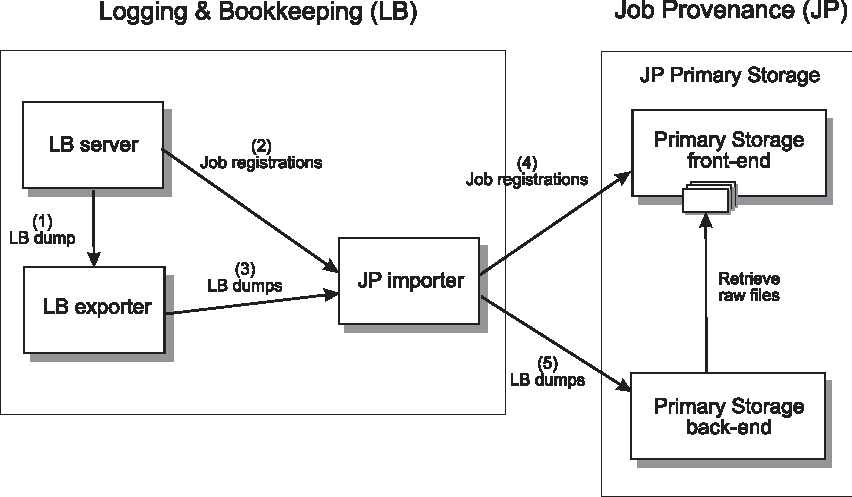
\includegraphics[width=0.9\hsize]{LB-JP-interaction-details}
  \caption{LB to JP interactions detail overview}
  \label{fig:LB-JP-interactions}
\end{figure}

\begin{table}[htpb]
 \centering
  \begin{tabular}{|c|l|l|p{9cm}|}
    \hline
    &spool directory&initiated by&description\\
    \hline
    \hline
    1&lb.export.dump&lb-exporter&Export of LB job records into spool 
    directory. It use glite-lb-purge utility. LB-exporter reads this
    spool directory
    in a regular manner and implement next processing of LB dumps.\\
    \hline
    2&lb.export.jpreg&LB server&When new job come to the LB server 
    it stores its
    registration into the spool directory. It is responsibility of
    JP-importer process to handle such registrations.\\
    \hline
    3&lb.export.jpdump&lb-exporter&LB-exporter do its processing of 
    LB dumps and passes
    on it to the JP-importer using the spool directory.\\
    \hline
    4&none&jp-importer&JP importer handles registrations received from LB
    server and sends it to the JP primary server front-end (using its WS
    interface).\\
    \hline
    5&none&jp-importer&JP importer handles LB dumps received from LB
    exporter and sends it to the JP primary server back-end using its
    gridftp interface.\\
    \hline
  \end{tabular}
  \caption{LB to JP data flows description}
  \label{tab:LB-JP-interactions}
\end{table}


Notes:
\begin{itemize}
 \item Only JP Primary Storage (JPPS) server is involved in described
   data flows. JP Index Servers are not part of this picture (they are
   feeded via corresponding JPPS).
 \item Only flows number 4 and 5 are designed to be inter-host. All
   the other interactions assume the components are on the same host and
   do use access to a shared filesystem.
 \item Data flow number 1 use glite-lb-purge utility (see its
   documentation) and passes to it argument from lb.export.purgeargs
   clause of the deployment configuration file. This argument contain
   the timeouts controlling after how long period of time a job
   staying in a terminal state is to be purged from the LB server.
 \item The LB exporter have a feature to store LB job event dumps in a
   directory for further handling (e.g. for job statistic tool). This behaviour
   is controled by lb.export.jobs deployment config file clause (leave
   this clause empty if you don't use dumps for futher handling).
 \item The LB exporter also have a feature to keep all handled LB
   dumps (in glite-lb-purge format) in filesystem. This feature is
   controlled by lb.export.dump.keep.
 \item LB exporter is not a deamon, it's periodic invocation is
   provided by cron deamon.
\end{itemize}

\end{document}
